
\subsection*{Código}
A execução dos códigos devem ser dados na seguinte forma:

As seguintes rotinas geram os sinais binários e quaternários, respectivamente e geram o diagrama de olho para os sinais livres de distorção. 
\begin{lstlisting}[language=Matlab,style=consolestyle]
>> eye_1.m 
>> eye_2.m
\end{lstlisting}

A aplicação das distorções pelo canal customizado só podem ser feitas após a execução das rotinas anteriores, pois elas fornecem as formas de onda para cada formatação de pulso.

\begin{lstlisting}[language=Matlab,style=consolestyle]
>> apply_channel.m
\end{lstlisting}

O canal customizado possui as seguintes características:

\begin{itemize}
    \item Aplicação de AWGN por meio de SNR fornecida;
    \item Aplicação de atraso temporal como uma fração aleatória do tempo de símbolo (o atraso se apresenta como um atraso único ou consecutivos atrasos para cada símbolo);
    \item Aplicação de desvio de frequência e fase aleatórios por meio de uma portadora complexa;
    \item Aplicação de um filtro que modela um canal telefônico, fornecido por Haykin ("Haykin, S., Moher, M., "Sistemas de Comunicação", 5a Edição, Editora Bookman, 2011.");
    \item Aplicação do modelo de canal de Rayleigh e Rician fornecido pela \textit{toolbox} de comunicações do MATLAB com propriedades semi-aleatórias.
\end{itemize}

O código fonte permite que qualquer uma dessas características sejam implementadas facilmente e podem ser cumulativas. Vide abaixo alguns exemplos de aplicação (o código apply\_channel.m possui algumas predefinições):

\begin{lstlisting}[language=Matlab,style=consolestyle]
>> SNR = signal_to_noise_ratio; % [dB]
>> SPS = sample_per_symbol;
>> in = input_message;
>> out1 = kanal(in,SNR,SPS,'awgn','delay','jitter','shift','telephone','rayleigh','rician');
>> out2 = kanal(in,SNR,SPS);
>> out3 = kanal(in,SNR,SPS,'awgn','jitter');
>> out4 = kanal(in,SNR,SPS,'shift','rician','awgn');
>> out5 = kanal(in,SNR,SPS,'rayleigh');
>> out6 = kanal(in,SNR,SPS,'delay','jitter','telephone');
\end{lstlisting}

OBS: A ordem dos três primeiros argumentos deve ser respeitadas, enquanto que os demais efeitos podem ser adicionados em qualquer ordem.

\subsection*{Comparação binária}

A título de comparação dos diagramas gerados, serão utilizadas diferentes combinações de degradações para os diferentes formatos de pulso (RZ, NRZ, \textit{half sine}, \textit{raised cosine}). Para o AWGN, foi considerado uma SNR fixa de 30 dB e para os demais efeitos que geram um sinal complexo, foi considerada apenas a parte real para o traçado do diagrama de olho.

\begin{figure}[H]
\begin{center}
    \subfigure[Pura]{             
        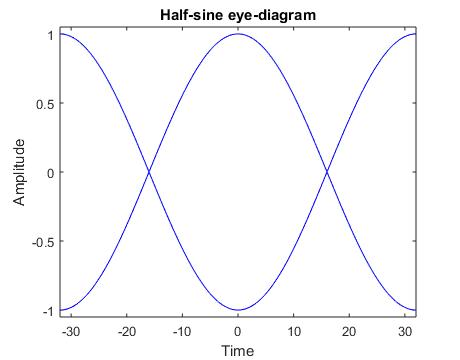
\includegraphics[width=7.5cm]{images/half_sine_pure.jpg}  
        \label{fig:1a}
    }
    \subfigure[AWGN + delay + jitter + canal telefônico]{                                              
        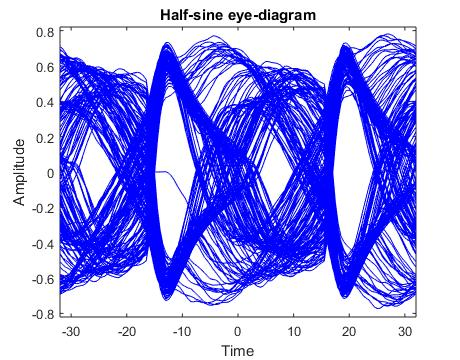
\includegraphics[width=7.5cm]{images/half_sine_deg.jpg}
        \label{fig:1b}
    }                
\end{center}
\caption{Comparação entre diagrama de olho para um sinal formatado com pulso \textit{half sine}.}
\label{fig:1} 
\end{figure}

Para o \textit{half sine} observa-se que o instante ótimo de amostragem foi prejudicado, restando janelas curtas de tempo para uma boa amostragem. Mesmo assim o limite de amplitude foi prejudicado pelo ruído.

\begin{figure}[H]
\begin{center}
    \subfigure[Pura]{             
        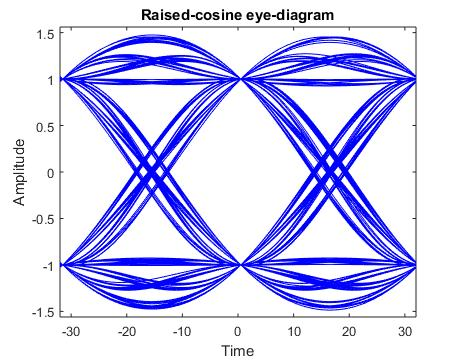
\includegraphics[width=7.5cm]{images/rcos_pure.jpg}  
        \label{fig:2a}
    }
    \subfigure[Desvio em fase e frequência]{                                              
        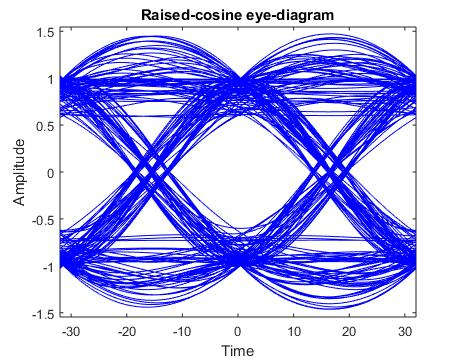
\includegraphics[width=7.5cm]{images/rcos_deg.jpg}
        \label{fig:2b}
    }                
\end{center}
\caption{Comparação entre diagrama de olho para um sinal formatado com pulso \textit{raised cosine}.}
\label{fig:2} 
\end{figure}

A inserção de um vetor girante no pulso \textit{raised cosine} se mostrou extremamente prejudicial para a ISI. Apesar do vetor inserido possuir rotação de 0.1\% da taxa de símbolo do sinal, valores maiores (e.g. 1\%) podem comprometer completamente a detecção do sinal

\begin{figure}[H]
\begin{center}
    \subfigure[Pura]{             
        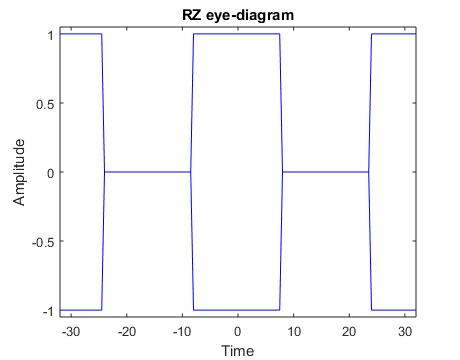
\includegraphics[width=7.5cm]{images/rz_pure.jpg}  
        \label{fig:3a}
    }
    \subfigure[AWGN + delay + canal telefônico]{                                              
        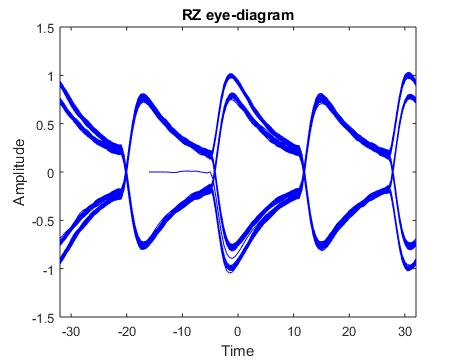
\includegraphics[width=7.5cm]{images/rz_deg.jpg}
        \label{fig:3b}
    }                
\end{center}
\caption{Comparação entre diagrama de olho para um sinal formatado com pulso RZ.}
\label{fig:3} 
\end{figure}

No caso RZ o canal telefônico possui características de atenuação, prejudicando o \textit{slope} ideal do formato do pulso. Porém, mesmo com os efeitos, o sinal ainda possui uma boa sensibilidade a amplitude, mas com certo cuidado no instante de amostragem, devido ao \textit{slope}.

\begin{figure}[H]
\begin{center}
    \subfigure[Pura]{             
        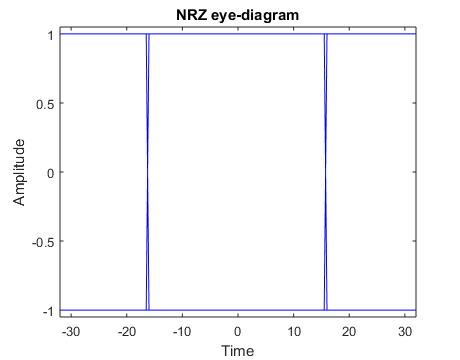
\includegraphics[width=7.5cm]{images/nrz_pure.jpg}  
        \label{fig:4a}
    }
    \subfigure[AWGN + Rician + Rayleigh]{                                              
        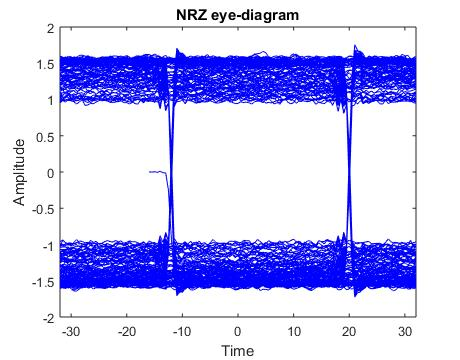
\includegraphics[width=7.5cm]{images/nrz_deg.jpg}
        \label{fig:4b}
    }                
\end{center}
\caption{Comparação entre diagrama de olho para um sinal formatado com pulso NRZ.}
\label{fig:4} 
\end{figure}

Para o sinal NRZ, as propriedades inseridas de desvanecimento de multi caminho dos canais Rayleigh e Rician contribuíram, juntamente com o leve AWGN, para reduzir a abertura máxima do olho. Porém, devido a uniformidade do NRZ, não será necessário ajustar o tempo de amostragem ideal.

\subsection*{Comparação quaternária}

Repetindo os mesmos testes e com as mesmas condições para o caso M-ário (M=4), obtém-se condições ainda mais destrutivas devido ao acúmulo de diferentes símbolos.

\begin{figure}[H]
\begin{center}
    \subfigure[Pura]{             
        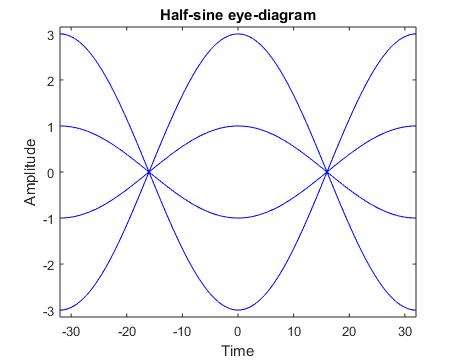
\includegraphics[width=7.5cm]{images/half_sine_pure_M.jpg}  
        \label{fig:5a}
    }
    \subfigure[AWGN + delay + jitter + canal telefônico]{                                              
        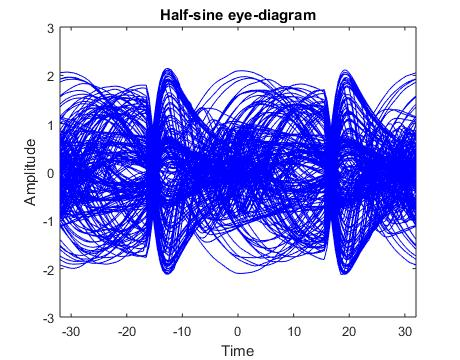
\includegraphics[width=7.5cm]{images/half_sine_deg_M.jpg}
        \label{fig:5b}
    }                
\end{center}
\caption{Comparação entre diagrama de olho para um sinal formatado com pulso \textit{half sine} M-ário (M=4).}
\label{fig:5} 
\end{figure}

\begin{figure}[H]
\begin{center}
    \subfigure[Pura]{             
        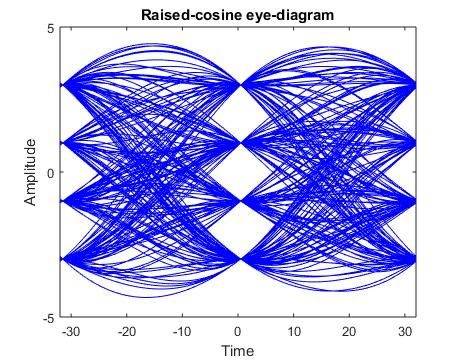
\includegraphics[width=7.5cm]{images/rcos_pure_M.jpg}  
        \label{fig:6a}
    }
    \subfigure[Desvio em fase e frequência]{                                              
        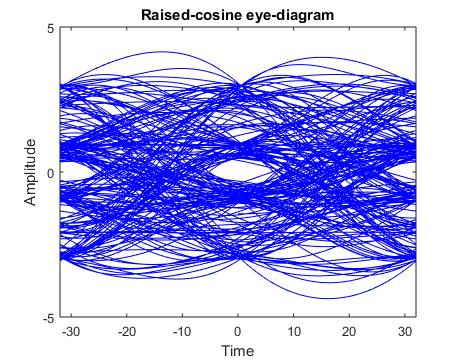
\includegraphics[width=7.5cm]{images/rcos_deg_M.jpg}
        \label{fig:6b}
    }                
\end{center}
\caption{Comparação entre diagrama de olho para um sinal formatado com pulso \textit{raised cosine} M-ário (M=4).}
\label{fig:6} 
\end{figure}


\begin{figure}[H]
\begin{center}
    \subfigure[Pura]{             
        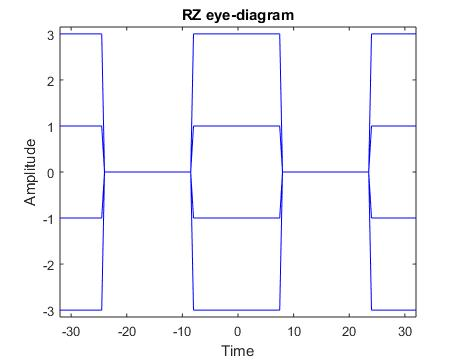
\includegraphics[width=7.5cm]{images/rz_pure_M.jpg}  
        \label{fig:7a}
    }
    \subfigure[AWGN + delay + canal telefônico]{                                              
        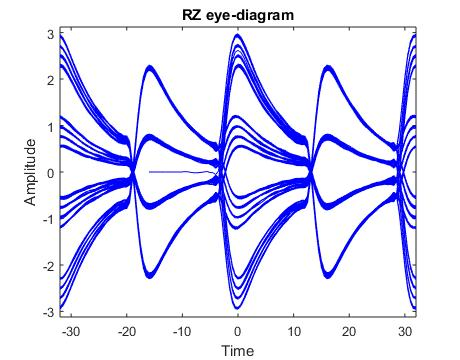
\includegraphics[width=7.5cm]{images/rz_deg_M.jpg}
        \label{fig:7b}
    }                
\end{center}
\caption{Comparação entre diagrama de olho para um sinal formatado com pulso RZ M-ário (M=4).}
\label{fig:7} 
\end{figure}


\begin{figure}[H]
\begin{center}
    \subfigure[Pura]{             
        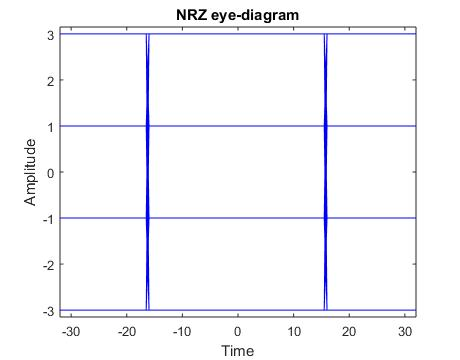
\includegraphics[width=7.5cm]{images/nrz_pure_M.jpg}  
        \label{fig:8a}
    }
    \subfigure[AWGN + Rician + Rayleigh]{                                              
        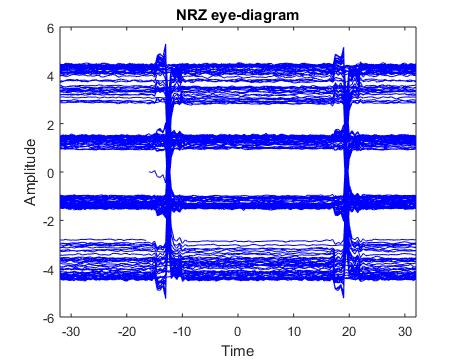
\includegraphics[width=7.5cm]{images/nrz_deg_M.jpg}
        \label{fig:8b}
    }                
\end{center}
\caption{Comparação entre diagrama de olho para um sinal formatado com pulso NRZ M-ário (M=4).}
\label{fig:8} 
\end{figure}

Os detalhes que podem ser discutidos são:

\begin{itemize}
    \item No caso do \textit{raised cosine} o sinal foi quase que em sua totalidade prejudicado, restando apenas um estreito olho, com um curto intervalo de amplitude e tempo de amostragem;
    \item Para o RZ, o canal telefônico gerou padrões de ISI mais complexos para maiores amplitudes, podendo prejudicar uma pouco mais a detecção dos símbolos do que no caso binário;
    \item O sinal NRZ possui um olho mais fechado devido ao AWGN e desvanecimento, mas isso só foi acentuado devido à interferência dos símbolos de diferentes amplitudes entre si;
    \item Finalmente o \textit{half sine} se mostrou bastante degradado para as mesmas condições que o caso binário.
\end{itemize}

Os efeitos que os sinais estão submetidos no canal são diversos e variam de acordo com o tipo de canal. Esses exemplos não procuram estabelecer um modelo de canal real, mas apenas combinar diversas degradações que podem ou não ocorrer juntas, com o objetivo de prejudicar o diagrama de olho e buscar um melhor entendimento da sua premissa.